\documentclass[../mit-general-chemistry.tex]{subfiles}
\begin{document}





\chapter{The shape of molecules}

The shape (geometry) of molecules influence physical and chemical
properties such as melting point, boiling point and reactivity. We saw
earlier that this made \ce{H2O} polar and \ce{CO2} non-polar.

When we talk about biology, shape is really important when we consider
enzymes having an active site where a molecule have to fit perfectly
into the active site and do so because of it's shape.

\begin{example}
  The intestinal enzyme sucrase is a great example of this as it
  catalyses the hydrolysis of sucrose (table sugar) by having the active
  site perfectly embrace and bind to the the sucrose molecule. This puts
  stress on the bond between the sugar molecules and breaks it which
  enables the body to use them.
\end{example}

\begin{figure}[t]
  \begin{margincap}
    \begin{center}
      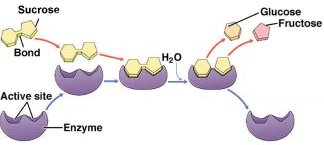
\includegraphics[width=.85\textwidth]{sucrase}
      \caption{
        The sucrase hydrolysis of sucrose is thouroughly dependent of
        shape of both the sucrose as well as the sucrase molecules as
        they have to fit precisely into eachothrt for the enzyme to
        work on the suger compound.
      }
    \end{center}
  \end{margincap}
\end{figure}







\section{Valence shell electron pair repulsion theory}

We are going to use VSEPR theory (valence shell electron pair
repulsion theory) figure out the shapes of molecules. VSEPR theory is
based on Lewis structures and the principles

\begin{itemize}
\item That electron pairs repel each other.
\item The geometry around the central atom will be such that the
  repulsion is minimized.
\end{itemize}

In VSEPR theory nomenclature \ce{A} denotes the central atom,
\ce{X} denotes bonded atoms and \ce{E} are lone electron pairs.

\paragraph{Steric number}
In VSEPR theory we need the concept of {\em steric numbers} of a
molecule. The steric number is the number of atoms that are bound To
the central atom plus the central atoms number of lone electron
pairs.

\begin{example}
  \ce{H2O} consists of a central oxygen atom bound to two hydrogen
  atoms. The oxygen atom also have two lone pairs of electrons.

  \begin{center}
    \chemfig{\lewis{1:3:,O}(-[:218]H)(-[:322]H)}
  \end{center}

  The steric number is $\stericnumber = 2 + 2 = 4$.
\end{example}

We do not consider the types of bonds in VSEPR theory, only the number
of bound atoms and lone pairs.


\paragraph{Resonance structures}
If a molecule has two or more resonance structures, the VSEPR model
can be applied to any one of them.


\begin{center}
\schemestart
  $\left[~
    \chemfig{\lewis{2:6:,O}=Cr(-[:90]\lewis{0:2:4:,O})(-[:270]\lewis{0:4:6:,O})=\lewis{2:6:,O}}
  ~\right]^{-2}$
\arrow{<->}
$\cdots$
\arrow{<->}
  $\left[~
    \chemfig{\lewis{2:4:6:,O}-Cr(=[:90]\lewis{0:4:,O})(=[:270]\lewis{0:4:,O})-\lewis{0:2:6:,O}}
  ~\right]^{-2}$
\schemestop
\end{center}





\paragraph{Multiple central atoms}
If there is more than one central atom in a molecule, consider the
bonding around each such atom separately.

\begin{center}
  \chemfig{H-\lewis{2:6:,O}-C(-[:90]H)(-[:270]H)-H}
\end{center}

In \ce{CH3OH} (methanol), both the carbon and the oxygen are considered
central atoms.


\begin{figure*}[t]
  \begin{center}
    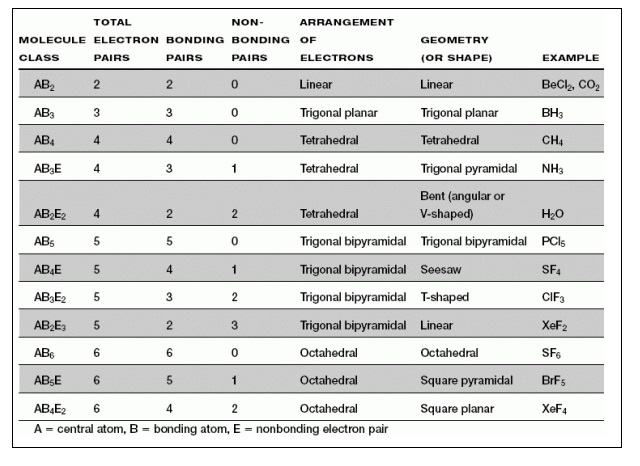
\includegraphics{vsepr1}
    \caption{Classes of molecules and their geometry (VSEPR theory).}
  \end{center}
\end{figure*}



Electrons in bonds have less ``spatial distribution'' than electrons in
lone pairs. This actually mean that electrons in bonds take up less
space. It also means that lone pairs take up more space and hence
experience more repulsion.

The most repulsive forces between electrons will be produced between
lone pair electrons. The least repulsive forces will be found between
bound electrons.


Lone pairs are axial or equatorial and that will affect the geometry
of the molecule. An axial lone pair will repel three bonding electron
pairs strongly, whereas a equatorial lone pair only affect two bonding
pairs to the same extent. An \ce{AX4E} molecule with an
equatorial lone pair take the shape of a sew-saw.


\ce{AX4E2} molecules are square planar. The two lone pairs are
farthest apart when they are on opposite sides of the central atom.






\subsubsection{Angles between bonded atoms}



For a tetrahedral molecules without any lone pairs (\ce{AX4}), the
bonding angles are $109.5^{\circ}$. tend to be smaller


Atom sizes increase as we go down a column of the periodic
table. Angles of bonded do however {\em decrease} as they are bound to
an element further down the periodic system group.








\section{Molecular orbital theory}


Lewis structures are very useful, they correctly predict bonding
between atoms over 90\% of the time. It is not correct all of the time
and the reason for this is that it's not based on quantum
theory. Molecular orbital theory is based on quantum theory.

In molecular orbital theory, MO theory, we use wave functions to
describe molecular orbitals. The wave functions of molecular orbitals
are linear combinations of atomic orbital wave functions.

In MO theory, valence electrons are delocalized over the entire
molecule, not confined to individual atoms or bonds. This means that
the electrons are spread out all over the molecule in the molecular
orbitals.






\subsection{Bonding and antibonding orbitals}

Molecular orbitals (wave functions) arise from adding together
(superimposing) atomic orbitals or wave functions. Remember that we
talk about wave functions and that we can have both constructive and
destructive interference.

Bonding orbitals, or molecular orbitals, are linear combinations of
atomic orbitals. In the illustration of this we see two atoms with one
$1s$ orbital each, form a $\sigma_{1s}$ orbital (which is a molecular
orbital) containing both nuclei.




\subsubsection{Bonding orbitals}


Bonding orbitals are, as we said, the result of constructive
interference between the wave functions of two atomic orbitals from
different atoms. When the $1s$ orbitals of the two atoms interfere the
result is a sigma orbital and they form a sigma bond
\begin{equation*}
  1s_a + 1s_b \longrightarrow \sigma_{1s}
\end{equation*}
$1s_a$ and $1s_b$ are the atomic $1s$ orbitals of atoms $a$ and
$b$. The sigma bond is a molecular orbital, electron density cloud,
that surrounds both nuclei of $a$ and $b$. The subscript in
$\sigma_{1s}$ means the molecular sigma orbital comes out of two $1s$
atomic orbitals.

Sigma bond orbitals are cylindrically symmetric along the bond axis
and there is no nodal plane along the bond axis. This is an important
criteria to remember later when we talk about $\sigma_{2p_z}$
orbitals and why the $2p_z$ orbitals produce sigma bonds.

For the probability density function there may be wave functions that
add to each other and wave functions that cancel each other out. When
the wave functions cancel each other out they create an antibonding
orbital. When constructive interference occur between the two wave
functions they create a bonding orbital.


For the probability density function (for finding an electron in a
certain position) we have $P \propto (\sigma_{1s})^2$ and since the
sigma orbital wave function is a linear combination of the two atomic
orbital wave functions we have
\begin{equation*}
  P \propto (\sigma_{1s})^2 = (1s_a + 1s_b)^2 = (1s_a)^2 + (1s_b)^2 + 2(1s_a)(1s_a)
\end{equation*}
where we see that $(1s_a)^2$ and $1s_b)^2$ are the probability
functions for the two atomic orbitals. The cross term $2(1s_a)(1s_a)$
represents constructive interference between the two atomic wave
functions.

In this case, where we're adding the functions together, this will be
constructive interference between the two $1s$ wave functions and this
will be what we are going to call a {\em bonding orbital}.


Let's consider the energy of interaction. The energy level of the
sigma orbital decreases compared to the atomic orbitals.


\begin{center}
  \begin{MOdiagram}[names,labels,labels-fs=\footnotesize]
    \atom[a]{left}{
      1s = {1; up},
    }
    \atom[b]{right}{
      1s = {1; up},
    }
    \molecule{
      1sMO = {0.5; pair }
    }
    \EnergyAxis[title=$E$]
  \end{MOdiagram}
\end{center}


From the diagram we immediately see that the electrons are more stable
than they were in the atoms, since they are at a lower energy
level. That is the idea of a bonding molecular orbital.









\subsubsection{Anti-bonding orbitals}


Now, since we are talking about wave functions and properties of
waves, they do not only have constructive interference they can also
have destructive interference.

In that case we would have one $1s_a$ and one $1s_b$ and subtract one
from the other


\begin{equation*}
  1s_a - 1s_b \longrightarrow \sigma^*_{1s}
\end{equation*}

which would give us a new wave function for this orbital (describing
an electron cloud) between those atoms. What we would see here is that
instead of us seeing ``more wave function'' in between the atoms, they
cancel each other out and we end up with a node. We are going to call
this new orbital $\sigma^*_{1s}$. The star, or asterisk, tells us this
is an anti-bonding orbital.

\begin{equation*}
  P \propto (\sigma_{1s})^2 = (1s_a - 1s_b)^2 = (1s_a)^2 + (1s_b)^2 - 2(1s_a)(1s_a)
\end{equation*}


\begin{remark}
  I'm thinking that when the two atoms bond the atomic orbitals form
  the molecular orbitals. Then the electrons from the two atoms'
  valence shell orbitals are redistributed among those molecule
  orbitals. Those electrons that end up in bonding orbitals strengthen
  the bond whereas the electrostatic forces stemming from electrons in
  anti-bonding orbtals weaken the bond.
\end{remark}


The energy increases compared to the atomic orbitals (by being less
negative).


$\sigma^*_{1s}$ is an anti-bonding orbital. This means that less
electron density accumulates between nuclei.


\begin{center}
  \begin{MOdiagram}[names,labels,labels-fs=\footnotesize]
    \atom[a]{left}{ 1s = {1; pair}, }
    \atom[b]{right}{ 1s = {1; pair}, }
    \molecule{ 1sMO = {.75/.75; pair, pair } }
    \EnergyAxis[title=$E$]
  \end{MOdiagram}
\end{center}

This is ``worse'' than non-bonding. Since we're gettinr rid of
electron density between the nuclei and we know that it is the
electron density that holds the two atoms together in a bond.

Anto-bonding creates an effect that is the {\em opposite} of a
bond. Anti-bonding is not non-bonding. Since the $\sigma^*_{1s}$
increases the energy level (less negative) of the two electrons this
is an unstable state.

The amount of energy that the energy is risen by in an anti-bonding
orbital energy level is the same amount that it is lowered by in a
bonding orbital.








\subsection{Homonuclear diatomic molecules}





\subsubsection{Molecules with MOs originating from $s$ orbitals}



Consider \ce{H2} with each atom having the electron configuration
$1s^1$. The \ce{H} atom is depicted in the following energy orbital
diagram

\begin{center}
  \begin{MOdiagram}[names,labels,labels-fs=\footnotesize]
    \atom[a]{left}{ 1s = {1; up}, }
    \EnergyAxis[title=$E$]
  \end{MOdiagram}
\end{center}

When two \ce{H} atoms form \ce{H2}
\ceeqstar{2H -> H2}
we get

\begin{center}
  \begin{MOdiagram}[names,labels,labels-fs=\footnotesize]
    \atom[\ce{H}]{left}{ 1s = {1; up}, }
    \atom[\ce{H}]{right}{ 1s = {1; up}, }
    \molecule[\ce{H2}]{ 1sMO = {.75/.75; pair } }
    \EnergyAxis[title=$E$]
  \end{MOdiagram}
\end{center}


We can see from the diagram above that the bond yields a net lowering
of the energy of the atoms.

We have written the electron configuration for atoms before. Now we
can do the same for molecules The electron configuration of \ce{H2} is
\begin{equation*}
  \ce{H2}: (\sigma_{1s})^2
\end{equation*}



In the same way we can fill in an energy level diagram for the
\ce{He2} molecule. We have a total of four valence electrons from the
two helium atoms so the reaction
\ceeqstar{2He -> He2}
give us the following energy diagram (we fill up molecular orbitals in
a similar way as we fill up atomic orbitals, one level at a time)

\begin{center}
  \begin{MOdiagram}[names,labels,labels-fs=\footnotesize]
    \atom[\ce{He}]{left}{ 1s = {1; pair}, }
    \atom[\ce{He}]{right}{ 1s = {1; pair}, }
    \molecule[\ce{He2}]{ 1sMO = {.75/.75; pair, pair } }
    \EnergyAxis[title=$E$]
  \end{MOdiagram}
\end{center}

We can write the electron configuration for molecular helium
\begin{equation*}
  \ce{He2}: (\sigma_{1s})^2(\sigma^*_{1s})^2
\end{equation*}

Because we do not have any net gain or gain loss in energy from
forming the bond between the two atoms. MO theory predicts that
\ce{He2} do not exist. We can figure this out using the concept of
bond order. In MO theory {\em bond order} (\bondorder) is
\begin{equation*}
  \bondorder = \frac{n_b - n_{a}}{2}
\end{equation*}
where $n_b$ is the number of electrons in bonding orbitals and $n_{a}$
is the number of electrons in anti-bonding orbitals. The bond order
tells us the nature of the bond between the atoms. Bond order can be zero
which means no bond, it can be one which means a single bond. A value
of one-and-a-half means a one-and-a-half bond, a value of two means a
double bond and so on.

For molecular helium we have $\bondorder = \frac{2 - 2}{2} = 0$ which
tells us that it is not a stable bond and this predicts that molecular
helium do not exist. \ce{He2} do in fact exist but the bond between
the atom is the weakest bond known and was not discovered until
1992. It is the weakest bond known and it has $\dissociationenergy =
\SI{0.01}{\kilo\joule\per\mol}$ whereas for molecular hydrogen we have
$\dissociationenergy = \SI{432}{\kilo\joule\per\mol}$ which is more
than \num{400000} times stronger.

For molecular hydrogen we have a bond order of $\bondorder = \frac{2 -
  0}{2} = 1$ which tells us that the \chemfig{H-H} bond is a single
bond.



If we continue through the periodic table we have lithium
next. Lithium have the electron configuration $1s^22s^1$ and the
formation of \ce{Li2}
\ceeqstar{2Li -> Li2}
gives us the orbital energy level diagram

\begin{center}
  \begin{MOdiagram}[names,labels,labels-fs=\footnotesize]
    \atom[\ce{Li}]{left}{ 1s = {1; pair}, 2s = {4; up}, }
    \atom[\ce{Li}]{right}{ 1s = {1; pair}, 2s = {4; up}, }
    \molecule[\ce{Li2}]{ 1sMO = {.75/.75; pair, pair }, 2sMO = {.75/.75; pair} }
    \EnergyAxis[title=$E$]
  \end{MOdiagram}
\end{center}

The bond order for this molecule is $\bondorder = \frac{4 - 2}{2} = 1$
so MO theory predicts that this is a stable molecule of two atoms with
a single bond. For \ce{Li2} we have $\dissociationenergy =
\SI{105}{\kilo\joule\per\mol}$





Beryllium has four electrons ($1s^22s^2$) and for \ce{Be2} we have
eight electrons for the two sigma orbitals formed which gives us the
diagram


\begin{center}
  \begin{MOdiagram}[names,labels,labels-fs=\footnotesize]
    \atom[\ce{Be}]{left}{ 1s = {1; pair}, 2s = {4; pair}, }
    \atom[\ce{Be}]{right}{ 1s = {1; pair}, 2s = {4; pair}, }
    \molecule[\ce{Be2}]{ 1sMO = {.75/.75; pair, pair }, 2sMO = {.75/.75; pair, pair} }
    \EnergyAxis[title=$E$]
  \end{MOdiagram}
\end{center}

We calculate $\bondorder = \frac{4 - 4}{2} = 0$ so MO theory predicts
that \ce{Be2} does not exist.



You don't have to consider all electrons in MO theory. In fact, you
don't have consider any core electrons, only valence electrons. In our
case, the diagram above can just as well be simplified to

\begin{center}
  \begin{MOdiagram}[names,labels,labels-fs=\footnotesize]
    \atom[\ce{Be}]{left}{ 2s = {1; pair}, }
    \atom[\ce{Be}]{right}{ 2s = {1; pair}, }
    \molecule[\ce{Be2}]{ 2sMO = {.75/.75; pair, pair} }
    \EnergyAxis[title=$E$]
  \end{MOdiagram}
\end{center}

which will give the same bond order $\bondorder = \frac{2 - 2}{2} = 0$
and we will make the same prediction.

The \chemfig{Be-Be} bond is in fact very weak, $\dissociationenergy
= \SI{9}{\kilo\joule\per\mol}$ which is very weak and so essentially
we're not going to see this.










\subsubsection{Molecules with MOs originating from $s$ and $p$ orbitals}


So far we have looked only on atoms with electrons in $s$
orbitals. Now as we go further we are going to look at atoms from the
$p$ block.

As we defined the sigma orbital wave functions from linear
combinations of the $s$ orbital wave functions we now denote molecular
orbitals from a linear combination of the $p_x$ and $p_y$ orbital wave
functions as $\pi_{2p_x}$ and $\pi_{2p_y}$ molecule orbitals formed
from $2p_x$ and $2p_y$ respectively. The pi bonds is formed from
parallel $p_x$ orbitals or from parallel $p_y$ orbitals.

Pi orbitals are molecular orbitals with a nodal plane through the bond
axis. This creates a space with sparse electron density. This comes
from the fact that the $z$ axis is the bond axis between atoms and
this makes the $p$ orbitals orthogonal to the bond axis.
\begin{equation*}
  2p_{xa} + 2p_{xb} \longrightarrow \pi_{2x_b}
\end{equation*}

The probability density function for pi bonds is
\begin{equation*}
  P \propto (\pi_{2p_x})^2 = (2p_{ax} + 2p_{bx})^2
  = (2p_{ax})^2 + (2p_{bx})^2 + 2(2p_{ax})(2p_{bx})
\end{equation*}
and again, $2(2p_{ax})(2p_{bx})$ is the interference term.

As in the sigma bonding/anti-bonding orbitals there is also pi
anti-bonding orbitals.

The pi anti-bonding orbitals are formed from $p$ orbitals facing
each other with destructive interference.
\begin{equation*}
  2p_{xa} - 2p_{xb} \longrightarrow \pi^*_{2x_b}
\end{equation*}

The probability density function for pi bonds is
\begin{equation*}
  P \propto (\pi_{2p_x})^2 = (2p_{ax} - 2p_{bx})^2
  = (2p_{ax})^2 + (2p_{bx})^2 + 2(2p_{ax})(2p_{bx})
\end{equation*}
The interference term has a negative sign and this means it describes
the destructive interference between the two $p$ orbitals. 

The $\pi^*$ orbitals result from destructive interference between the
$p_x$ orbitals and between the $p_y$ orbitals.

This makes it possible for us to consider boron (\ce{B}) which have
the electron configuration $1s^22s^22p^1$. Boron and \ce{B2} gives the
energy level diagram

\begin{center}
  \begin{MOdiagram}[names,labels,labels-fs=\footnotesize]
    \atom[\ce{B}]{left}{ 2s, 2p = {; up} }
    \atom[\ce{B}]{right}{ 2s, 2p = {; up} }
    \molecule[\ce{B2}]{ 2sMO, 2pMO = {; up, up} }
    \EnergyAxis[title=$E$]
  \end{MOdiagram}
\end{center}

With reservations for the latex modiagram package, we get a valence
electron configuration $\ce{B2}:
(\sigma_{2s})^2(\sigma^*_{2s})^2(\pi_{2x})^1(\pi_{2y})^1$. We also
have $\bondorder = \frac{1}{2}(4 - 2) = 1$.

Now we investigate carbon which have four valence electrons.


\begin{center}
  \begin{MOdiagram}[names,labels,labels-fs=\footnotesize]
    % left atom
    \AO[2sleft](1cm){s}[label={$2s_{2}$}]{1;pair} %AO1
    \AO(1cm){s}[label={$2p_x$}]{5;up}
    \AO(1.5cm){s}[label={$2p_y$}]{5;up}
    \AO[2pzleft](2cm){s}[label={$2p_z$}]{5;}    
    \node at (1cm, -1){\ce{C}};

    % right atom
    \AO[2sright](7cm){s}[label={$2s$}]{1;pair} % AO3
    %\AO(7cm){p}[label[x]={$2p_x$},label[y]={$2p_y$},label[z]={$2p_z$}]{5;up,up}
    \AO[2pxright](6.5cm){s}[label={$2p_x$}]{5;up}
    \AO(7cm){s}[label={$2p_y$}]{5;up}
    \AO(7.5cm){s}[label={$2p_z$}]{5;}    
    \node at (7cm, -1){\ce{C}};

    % molecule
    \AO[sigma2](4.5cm){s}[label={$\sigma_{2s}$}]{0.5;pair} % AO5
    \AO[sigma2*](4.5cm){s}[label={$\sigma^*_{2s}$}]{1.5;pair}
    \AO[pi2x](4.2cm){s}[label={$\pi_{2px}$}]{4;pair} % AO7
    \AO[pi2y](4.8cm){s}[label={$\pi_{2py}$}]{4;pair}
    \AO(4.5cm){s}[label={$\sigma_{2pz}$}]{3;}

    \AO[pi2x*](4.2cm){s}[label={$\pi^*_{2px}$}]{7;} % AO10
    \AO[pi2y*](4.8cm){s}[label={$\pi^*_{2py}$}]{7;}
    \AO(4.5cm){s}[label={$\sigma^*_{2pz}$}]{8;}
    \node at (4.5cm, -1){\ce{C2}};

    \draw[densely dotted,draw=black] (2sleft.0) -- (sigma2.180);
    \draw[densely dotted,draw=black] (2sleft.0) -- (sigma2*.180);
    \draw[densely dotted,draw=black] (2sright.180) -- (sigma2.0);
    \draw[densely dotted,draw=black] (2sright.180) -- (sigma2*.0);
    
    \draw[densely dotted,draw=black] (2pzleft.0) -- (pi2x.180);
    \draw[densely dotted,draw=black] (2pxright.180) -- (pi2y.0);
    \draw[densely dotted,draw=black] (2pzleft.0) -- (pi2x*.180);
    \draw[densely dotted,draw=black] (2pxright.180) -- (pi2y*.0);

    \EnergyAxis[title=$E$]
  \end{MOdiagram}
\end{center}

Dicarbon has the electron configuration
$(\sigma_{2s})^2(\sigma^*_{2s})^2(\pi_{2px})^2(\pi_{2py})^2$ and
$\bondorder = \frac{1}{2}(6 - 2) = 2$. So \ce{C2} have a double bond
\chemfig{C=C}.



Now, we are going to look at $p_z$ orbitals and the molecular orbitals
they form. When two $p_z$ orbitals form a bond we remember that the
orbitals are aligned with the $z$-axis, the internuclear axis, and so
this is a sigma bond. Since this bond orbital is cylindrically
symmetric along the bond axis and there is no nodal plane along the
bond axis, this is in fact a sigma orbital. Two $p_z$ orbitals form a
$\sigma_{p_z}$ orbital when bonding.
\begin{equation*}
  2p_{za} + 2p_{zb} \longrightarrow \sigma_{2p_z}\qquad\text{(constructive interference)}
\end{equation*}

We can also talk about anti-bonding orbitals when we have destructive
interference. We write this for the $2p_z$ of two atoms $a$ and $b$
\begin{equation*}
  2p_{za} - 2p_{zb} \longrightarrow \sigma^*_{2p_z}\qquad\text{(destructive interference)}
\end{equation*}

The two $p$ orbitals still form a sigma bond. The orbital have a nodal
plane in the middle where the two probability density functions cancel
each other out, but the internuclear axis is orthogonal to the nodal
plane so this is still a sigma bond.

Lets look at a diatomic molecule for atoms with electrons in the
$2p_z$ orbital. Lets look at molecular oxygen, \ce{O2}. The oxygen
atom have the electron configuration $1s^22s^22p^4$. The molecular
orbital diagram for molecular oxygen becomes



\begin{center}
  \begin{MOdiagram}[names,labels,labels-fs=\footnotesize]
    % left atom
    \AO[2sleft](1cm){s}[label={$2s_{2}$}]{1;pair} %AO1
    \AO[2pxleft](1.5cm){s}[label={$2p_x$}]{5;pair}
    \AO[2pyleft](2cm){s}[label={$2p_y$}]{5;up}
    \AO[2pzleft](1cm){s}[label={$2p_z$}]{5;up}    
    \node at (1cm, -1){\ce{O}};

    % right atom
    \AO[2sright](7cm){s}[label={$2s$}]{1;pair} % AO3
    \AO[2pxright](6.5cm){s}[label={$2p_x$}]{5;pair}
    \AO[2pyright](7cm){s}[label={$2p_y$}]{5;up}
    \AO[2pzright](7.5cm){s}[label={$2p_z$}]{5;up}
    \node at (7cm, -1){\ce{O}};

    % molecule
    \AO[sigma2](4.5cm){s}[label={$\sigma_{2s}$}]{0.5;pair} % AO5
    \AO[sigma2*](4.5cm){s}[label={$\sigma^*_{2s}$}]{1.5;pair}
    \AO[pi2x](4.2cm){s}[label={$\pi_{2p_x}$}]{4;pair} % AO7
    \AO[pi2y](4.8cm){s}[label={$\pi_{2p_y}$}]{4;pair}
    \AO[sigma2pz](4.5cm){s}[label={$\sigma_{2p_z}$}]{3;pair}

    \AO[pi2x*](4.2cm){s}[label={$\pi^*_{2p_x}$}]{7;up} % AO10
    \AO[pi2y*](4.8cm){s}[label={$\pi^*_{2p_y}$}]{7;up}
    \AO[sigma2pz*](4.5cm){s}[label={$\sigma^*_{2p_z}$}]{8;}
    \node at (4.5cm, -1){\ce{O2}};

    \draw[densely dotted,draw=black] (2sleft.0) -- (sigma2.180);
    \draw[densely dotted,draw=black] (2sleft.0) -- (sigma2*.180);
    \draw[densely dotted,draw=black] (2sright.180) -- (sigma2.0);
    \draw[densely dotted,draw=black] (2sright.180) -- (sigma2*.0);
    
    \draw[densely dotted,draw=black] (2pyleft.0) -- (pi2x.180);
    \draw[densely dotted,draw=black] (2pxright.180) -- (pi2y.0);
    \draw[densely dotted,draw=black] (2pyleft.0) -- (pi2x*.180);
    \draw[densely dotted,draw=black] (2pxright.180) -- (pi2y*.0);

    \draw[densely dotted,draw=black] (2pzleft.0) -- (sigma2pz*.180);
    \draw[densely dotted,draw=black] (2pzleft.0) -- (sigma2pz.180);
    \draw[densely dotted,draw=black] (2pzright.180) -- (sigma2pz*.0);
    \draw[densely dotted,draw=black] (2pzright.180) -- (sigma2pz.0);
    \EnergyAxis[title=$E$]
  \end{MOdiagram}
\end{center}

Molecular oxygen has $\bondorder = 2$, which suggests a double
bond. The \dissociationenergy is \SI{494}{\kilo\joule\per\mol}. The
two odd electrons in $\pi^*_{2p_x}$ and $\pi^*_{2p_y}$ makes \ce{O2} a
{\em biradical}. This is not something we could have predicted using
Lewis structures as that looks like this
\begin{center}
  \chemfig{\lewis{3:5:,O}=\lewis{1:7:,O}}
\end{center}
but becomes evident through molecular orbital theory.





An interesting piece of knowledge is shown when we look at nitrogen,
\ce{{}_7N}. For small enough elements, $Z < 8$, the energy level of
$\sigma_{2p_z}$ is higher (less negative) than the energy level of the
$\pi_{2p_x}$ and the $\pi_{2p_y}$ orbitals. For neutral species this
is only shown in molecular nitrogen, \ce{N2}, because of electron
configurations.

The molecular orbital diagram of \ce{N2} is shown below.


\begin{center}
  \begin{MOdiagram}[names,labels,labels-fs=\footnotesize]
    % left atom
    \AO[2sleft](1cm){s}[label={$2s_{2}$}]{1;pair} %AO1
    \AO[2pxleft](1.5cm){s}[label={$2p_x$}]{5;up}
    \AO[2pyleft](2cm){s}[label={$2p_y$}]{5;up}
    \AO[2pzleft](1cm){s}[label={$2p_z$}]{5;up}    
    \node at (1cm, -1){\ce{N}};

    % right atom
    \AO[2sright](7cm){s}[label={$2s$}]{1;pair} % AO3
    \AO[2pxright](6.5cm){s}[label={$2p_x$}]{5;up}
    \AO[2pyright](7cm){s}[label={$2p_y$}]{5;up}
    \AO[2pzright](7.5cm){s}[label={$2p_z$}]{5;up}
    \node at (7cm, -1){\ce{N}};

    % molecule
    \AO[sigma2](4.5cm){s}[label={$\sigma_{2s}$}]{0.5;pair} % AO5
    \AO[sigma2*](4.5cm){s}[label={$\sigma^*_{2s}$}]{1.5;pair}
    \AO[pi2x](4.2cm){s}[label={$\pi_{2p_x}$}]{3;pair} % AO7
    \AO[pi2y](4.8cm){s}[label={$\pi_{2p_y}$}]{3;pair}
    \AO[sigma2pz](4.5cm){s}[label={$\sigma_{2p_z}$}]{4;pair}

    \AO[pi2x*](4.2cm){s}[label={$\pi^*_{2p_x}$}]{7;} % AO10
    \AO[pi2y*](4.8cm){s}[label={$\pi^*_{2p_y}$}]{7;}
    \AO[sigma2pz*](4.5cm){s}[label={$\sigma^*_{2p_z}$}]{8;}
    \node at (4.5cm, -1){\ce{N2}};

    \draw[densely dotted,draw=black] (2sleft.0) -- (sigma2.180);
    \draw[densely dotted,draw=black] (2sleft.0) -- (sigma2*.180);
    \draw[densely dotted,draw=black] (2sright.180) -- (sigma2.0);
    \draw[densely dotted,draw=black] (2sright.180) -- (sigma2*.0);
    
    \draw[densely dotted,draw=black] (2pyleft.0) -- (pi2x.180);
    \draw[densely dotted,draw=black] (2pxright.180) -- (pi2y.0);
    \draw[densely dotted,draw=black] (2pyleft.0) -- (pi2x*.180);
    \draw[densely dotted,draw=black] (2pxright.180) -- (pi2y*.0);

    \draw[densely dotted,draw=black] (2pzleft.0) -- (sigma2pz*.180);
    \draw[densely dotted,draw=black] (2pzleft.0) -- (sigma2pz.180);
    \draw[densely dotted,draw=black] (2pzright.180) -- (sigma2pz*.0);
    \draw[densely dotted,draw=black] (2pzright.180) -- (sigma2pz.0);
    \EnergyAxis[title=$E$]
  \end{MOdiagram}
\end{center}


For \ce{N2}, $\bondorder = 3$ which suggests a triple bond between the
nitrogen atoms. This is also reflected in the dissasociation energy
which is \SI{941}{\kilo\joule\per\mol}.

The triple bond is also reflected in a properly calculated Lewis
structure. The nitrogen atoms have ten valence electrons between
them. We need 16 electrons to satisfy the octet rule for the
atoms. This tells us the atoms need to share $16 - 10 = 6$
electrons. If we follow this we get teh following Lewis structure

\begin{center}
  \chemfig{\lewis{4:,N}~\lewis{0:,N}}
\end{center}

The electron configuration for \ce{N2} is
\begin{equation*}
  \ce{N2}:
  (\sigma_{1s})^2
  (\sigma^*_{1s})^2
  (\sigma_{2s})^2
  (\sigma^*_{2s})^2
  (\pi_{2p_x})^2
  (\pi_{2p_y})^2
  (\sigma_{2p_z})^2
\end{equation*}




\subsection{Heteronuclear diatomic molecules}

So far, we have only discussed homonuclear molecules within molecular
orbital theory. Molecules that consists of two atoms of the same
element.

When we're talking about electrons within molecular orbitals we're
looking at electrons as waves. This makes us able to discuss them
having constructive as well as destructive interference






Consider carbonmonoxide, \ce{CO}.

\begin{center}
  \begin{MOdiagram}[names,labels,labels-fs=\footnotesize]
    % left atom
    \AO[2sleft](1cm){s}[label={$2s_{2}$}]{1;pair} %AO1
    \AO[2pxleft](1.5cm){s}[label={$2p_x$}]{5;up}
    \AO[2pyleft](2cm){s}[label={$2p_y$}]{5;up}
    \AO[2pzleft](1cm){s}[label={$2p_z$}]{5;}    
    \node at (1cm, -1){\ce{C}};

    % right atom
    \AO[2sright](7cm){s}[label={$2s$}]{1;pair} % AO3
    \AO[2pxright](6.5cm){s}[label={$2p_x$}]{5;pair}
    \AO[2pyright](7cm){s}[label={$2p_y$}]{5;up}
    \AO[2pzright](7.5cm){s}[label={$2p_z$}]{5;up}
    \node at (7cm, -1){\ce{O}};

    % molecule
    \AO[sigma2](4.5cm){s}[label={$\sigma_{2s}$}]{0.5;pair} % AO5
    \AO[sigma2*](4.5cm){s}[label={$\sigma^*_{2s}$}]{1.5;pair}
    \AO[pi2x](4.2cm){s}[label={$\pi_{2p_x}$}]{4;pair} % AO7
    \AO[pi2y](4.8cm){s}[label={$\pi_{2p_y}$}]{4;pair}
    \AO[sigma2pz](4.5cm){s}[label={$\sigma_{2p_z}$}]{3;pair}

    \AO[pi2x*](4.2cm){s}[label={$\pi^*_{2p_x}$}]{7;} % AO10
    \AO[pi2y*](4.8cm){s}[label={$\pi^*_{2p_y}$}]{7;}
    \AO[sigma2pz*](4.5cm){s}[label={$\sigma^*_{2p_z}$}]{8;}
    \node at (4.5cm, -1){\ce{CO}};

    \draw[densely dotted,draw=black] (2sleft.0) -- (sigma2.180);
    \draw[densely dotted,draw=black] (2sleft.0) -- (sigma2*.180);
    \draw[densely dotted,draw=black] (2sright.180) -- (sigma2.0);
    \draw[densely dotted,draw=black] (2sright.180) -- (sigma2*.0);
    
    \draw[densely dotted,draw=black] (2pyleft.0) -- (pi2x.180);
    \draw[densely dotted,draw=black] (2pxright.180) -- (pi2y.0);
    \draw[densely dotted,draw=black] (2pyleft.0) -- (pi2x*.180);
    \draw[densely dotted,draw=black] (2pxright.180) -- (pi2y*.0);

    \draw[densely dotted,draw=black] (2pzleft.0) -- (sigma2pz*.180);
    \draw[densely dotted,draw=black] (2pzleft.0) -- (sigma2pz.180);
    \draw[densely dotted,draw=black] (2pzright.180) -- (sigma2pz*.0);
    \draw[densely dotted,draw=black] (2pzright.180) -- (sigma2pz.0);
    \EnergyAxis[title=$E$]
  \end{MOdiagram}
\end{center}


We fill in the molecular orbitals in order of their energy level,
bottom-up. The electron configuration for \ce{CO} is
\begin{equation*}
  \ce{CO}:
  (\sigma_{1s})^2
  (\sigma^*_{1s})^2
  (\sigma_{2s})^2
  (\sigma^*_{2s})^2
  (\sigma_{2p_z})^2
  (\pi_{2p_x})^2
  (\pi_{2p_y})^2
\end{equation*}




The molecule have bond order, $\bondorder = 3$ and the dissociation
energy is \SI{1072}{\kilo\joule\per\mol}. The bondorder suggests a
triple bond, as in \ce{N2} which is consistent with experiments. The
huge dissociation energy is also consistent with a triple bond.





\section{Valence bond theory and hybridization}


In {\em valence bond theory}, bonds result from the pairing of unpaired
electrons from valence shell atomic orbitals.

The simplest case we can think of is the forming of nitrogen gas from
two hydrogen atoms
\ceeqstar{2H -> H2}
The two atoms have one valence electron in a $1s$ orbital each. The
atoms form a bond as the atoms come together.

In molecular orbital theory, we named orbitals based on their
symmetry. In valence bond theory the focus is on discussing the
bond. The bonds we are going to discuss are familiar to us. They are
sigma bonds and pi bonds.



\subsection{Sigma and pi bonds}


We have already seen earlier that sigma bonds are formed from two $s$
orbitals or two $p_z$ orbitals sharing electrons. We also know that th
pi bonds are formed from two $p_x$ or two $p_y$
orbitals aligning upp in parallel as the interaction occur between
each orbital's two lobes.



\begin{figure}[h]
  \begin{margincap}
    \begin{center}
      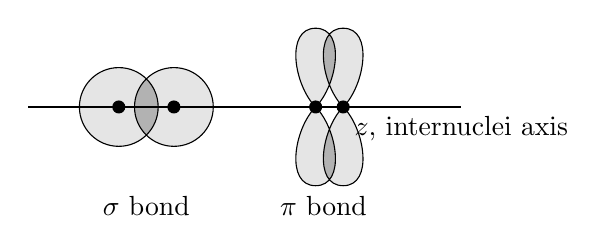
\begin{tikzpicture}[x=.5cm,y=.5cm]
        \def\firstellipse{(-.7,0) ellipse (1 and 1)}
        \def\secondellipse{(.7,0) ellipse (1 and 1)}
        \def\firstp{(O) to [out=135,in=180] (A10) to [out=0,in=45] (O) to [out=225,in=180] (A10m) to [out=0,in=-45] (O)}
        \def\secondp{(O1) to [out=135,in=180] (A11) to [out=0,in=45] (O1) to [out=225,in=180] (A11m) to [out=0,in=-45] (O1)}
        \coordinate (O) at (4.3,0,0);
        \coordinate (O1) at (5,0,0);
        \coordinate (A10) at (4.3,2,0);
        \coordinate (A11) at (5,2,0);
        \coordinate (A10m) at (4.3,-2,0);
        \coordinate (A11m) at (5,-2,0);

        % colour ellipses
        \fill[black!10] \firstellipse \secondellipse;
        \fill[black!10] \firstp \secondp;

        % colour intersection
        \begin{scope}
          \clip \firstellipse;
          \fill[black!30] \secondellipse;
        \end{scope}
        \begin{scope}
          \clip \firstp;
          \fill[black!30] \secondp;
        \end{scope}

        % outiline of ellipses
        \draw \firstellipse \secondellipse;
        \draw \firstp \secondp;
        \draw (-3, 0) -- (8, 0) node[at end, below]{$z$, internuclei axis};
        \node at (0, -2.5) {$\sigma$ bond};
        \node at (4.5, -2.5) {$\pi$ bond};

        \draw[black,fill=black] (O) circle (.5ex);
        \draw[black,fill=black] (O1) circle (.5ex);
        \draw[black,fill=black] (-.7,0) circle (.5ex);
        \draw[black,fill=black] (.7,0) circle (.5ex);
      \end{tikzpicture}
    \end{center}
    \caption{Sigma and Pi bonds between molecules.}
  \end{margincap}
\end{figure}




A sigma bond forms as two orbitals interact, ``head to head'', along
the bond axis. A sigma bond is symmetric about the bond axis and have
no nodal planes along the bond axis.

Pi bonds have electron density in two lobe above and below the bond
axis with a single nodal plane along the bond axis.

These are definitions and criteria for the two bond classes that we
used earlier when we discussed the $p_z/p_z$ bond in molecular orbital
theory.

The pi bonds seem to consist of two orbitals, but both darker regions
of the pi bond in the figure is part of the same molecular orbital and
the pi bond is in itself a single bond even though pi bonds are always
part of a double (or triple) bond.

Single, double and triple bonds ar combinations of sigma and pi
molecular orbitals, a.k.a. bonds. A single bonds consists of one sigma
bond, a double bond consists of one sigma bond and one pi bond. A
triple bond between two atoms consists of one sigma bond and two pi
bonds.



\subsection{Hybridization of atomic orbitals}



Now, let's consider methane, \ce{CH4}. This is going to cause us
problems at this point.

The simple valence bond theory approach can not be applied to
accurately describe bonding in certain polyatomic molecules, such as
methane, \ce{CH4}.


\begin{center}
  \begin{MOdiagram}[names,labels,labels-fs=\footnotesize]
    \atom[\ce{C}]{left}{
      2s = {.5;pair},
      2p = {2;up,up}
    }
    \EnergyAxis[title=$E$]
  \end{MOdiagram}
\end{center}


What would we predict from considering methane, using valence bonding
theory? We would expect the carbon to pair up it's unpaired electrons
in the $p$ orbitals with unpaired electrons in the hydrogen. That only
gives us two electrons available for bonding. But we know that carbon
is tetravalent.

Simple valence bonding theory predicts \ce{CH2} as a stable species
with a bond \chemfig{H-C-H} angle of $90^{\circ}$ (because of the
orthogonal $2p_x$ and $2p_y$ orbitals). We know this is all wrong and
thus falsifies the simple theory. So we have to tweak our reasoning
for this theory to hold.  If the theory is true, we expect carbon to
have four unpaired electrons and the way this is achieved is through
{\em electron promotion} and {\em hybridization}.






\subsubsection{$sp^3$ hybridization}




The reasoning leading up to the idea of electron promotion is that if
one of the $2s$ electrons were to be ``promoted'' up to the empty
$2p_z$ orbital, we would have four unpaired electrons (as we know is
the case).

Promoting the electron obviously cost energy, but not as much energy
as one might expect. Both of the pair of electrons from the $2s$
orbital will feel less electron repulsion once one of them are
promoted. This will not explain the process of hybridization but we
will leave that for now. Let's just assume that this happens.


Since electrons are waves, as we talk about wave functions, we can
constructively and destructively combine these waves, these atomic
orbitals to make hybrid orbitals.


\begin{center}
  \begin{MOdiagram}[names,labels,labels-fs=\footnotesize]
    % left atom
    \AO[2sleft](1cm){s}[label={$2s_{2}$}]{.5;pair} %AO1
    \AO[2pxleft](1.5cm){s}[label={$2p_x$}]{3;up}
    \AO[2pyleft](2cm){s}[label={$2p_y$}]{3;up}
    \AO[2pzleft](1cm){s}[label={$2p_z$}]{3;}    
    \node at (1cm, -1){\ce{C}};
    \node[align=center,text width=2cm] at (1cm, -1.5cm){four valence $e^-$};

    % right atom
    \AO[2sp31](5.7cm){s}[label={$2sp^3$}]{2;up} % AO3
    \AO[2sp32](6.4cm){s}[label={$2sp^3$}]{2;up}
    \AO[2sp33](7.1cm){s}[label={$2sp^3$}]{2;up}
    \AO[2sp34](7.8cm){s}[label={$2sp^3$}]{2;up}
    \node at (7cm, -1.5cm){\itshape Hybrid orbitals};

    \draw[ultra thick,->](3cm, 1cm) -- (5cm, 1cm)
      node[midway,below]{\scriptsize\itshape hybridization};
    \EnergyAxis[title=$E$]
  \end{MOdiagram}
\end{center}



Notice that the hybrid $sp^3$ orbitals are all the same energy
level. The are similar in every way except for their orientation in
space. The $sp^3$ orbitals are wave functions that is the result of
linear combinations of the original $2s, 2p_x, 2p_y$ and $2p_z$
orbitals.

By calling the hybridized orbitals $sp^3$ orbitals we acknowledge that
they are formed out of one $s$ orbital and three $p$ orbitals.

The shape of the $sp^3$ orbitals is neither that of the sphere nor the
dumbbell. It has two lobes of different size, like the dumbbell, but
one of the lobes is far larger where we the $p$ orbital lobe has
constructive interference with the sphere $s$ orbital and the other
lobe, where we have destructive interference with the $s$ orbital wave
function, the lobe is smaller.

If we combine the four $sp^3$ orbitals along a $x, y, z$ coordinate
system we get a tetrahedral of lobes consisting of the larger lobes of
the $sp^3$ orbitals with the smaller lobes hidden between them. The
angles between the axis of each of the orbitals is, of course,
$109.5^{\circ}$.


Returning to the methane molecule, the carbon now have the four
unpaired electrons to bond with the four hydrogen atoms. Finally, we
need to account for the energy for the electron promotion. The energy
comes from bonding. We have seen in molecular orbital theory and
through experiments that electrons in molecular orbitals have a lower
(more negative) energy level than they do in unbounded atoms.

In the case of methane, the energy from bonding with the four hydrogen
atoms more than emough compensate for the energy of promoting the
electron(s).

As the $2sp^3$ orbitals of the carbon interact with the $1s$ orbitals
of each hydrogen, the bonding orbital becomes a sigma orbital. The
bond axis is an axis between the two nuclei of the atoms involved in
the bonding. Each of the \chemfig{C-H} bonds of the molecule will be
called $\sigma(\ce{C}2sp^3\ce{H}1s)$, even though
$\sigma_{\ce{C}2sp^3\ce{H}1s}$ looks way smarter.



Now we can interest ourselves with more complicated molecules like
\ce{C2H6}, ethane. If we just turn our tetrahedron around and let the
two carbons bond with one each of their $2sp^3$ orbitals, there are
six spots free for hydrogen atoms to bind to. The bond between the
carbon atoms is, of course, a sigma bond. We do, however, have two
types of bonds in the ethane molecule.

Describing ethane with respect to the bonds and atoms of the molecule
we can write:
\begin{equation*}
  \ce{C2H6}:
  \sigma_{\ce{C}s2sp^3,\ce{C}s2sp^3}\sigma_{\ce{C}2sp^3,\ce{H}1s}
\end{equation*}

This is actually one fairly full description of the ethane molecule.



Electron promotion does {\em not} occur in nitrogen, \ce{N}, because
that would not increase the number of unpaired electrons.

It is, however, still possible that the $n_2$ shell orbitals hybridize
and form four $2sp^3$ orbitals.


\begin{center}
  \begin{MOdiagram}[names,labels,labels-fs=\footnotesize]
    % left atom
    \AO[2sleft](1cm){s}[label={$2s_{2}$}]{.5;pair} %AO1
    \AO[2pxleft](1.5cm){s}[label={$2p_x$}]{3;up}
    \AO[2pyleft](2cm){s}[label={$2p_y$}]{3;up}
    \AO[2pzleft](1cm){s}[label={$2p_z$}]{3;up}
    \node at (1cm, -1){\ce{N}};

    % right atom
    \AO[2sp31](5.7cm){s}[label={$2sp^3$}]{2;pair} % AO3
    \AO[2sp32](6.4cm){s}[label={$2sp^3$}]{2;up}
    \AO[2sp33](7.1cm){s}[label={$2sp^3$}]{2;up}
    \AO[2sp34](7.8cm){s}[label={$2sp^3$}]{2;up}
    \node at (7cm, -1cm){\itshape Hybrid orbitals};

    \draw[ultra thick,->](3cm, 1cm) -- (5cm, 1cm)
      node[midway,below]{\scriptsize\itshape hybridization};
    \EnergyAxis[title=$E$]
  \end{MOdiagram}
\end{center}


The hybridized nitrogen atom has three unpaired electrons and one
lonely pair, so the ammonia molecule, \ce{NH3}, has the triagonal
pyramidal geometry and the lonely pair on top decreases the bond
angles between the hydrogen atoms so it is less than $109.5^{\circ}$
(it is actually $107^{\circ}$).

The three \chemfig{N-H} bonds are similar to the \chemfig{C-H} bonds
of methane. They are $\sigma_{\ce{N}2sp^3,\ce{H}1s}$.








Let's talk about oxygen hybridization. Oxygen has six valence
electrons in $2s^22p_x^22p_y^12p_z^1$. Electron promotion is not
favored in oxygen since we're going to have two lone pairs no matter
what we do (as seen below).

Hybridized oxygen have four $2sp^3$ orbitals with two unpaired
electrons and two lone pairs.


\begin{center}
  \begin{MOdiagram}[names,labels,labels-fs=\footnotesize]
    % left atom
    \AO[2sleft](1cm){s}[label={$2s_{2}$}]{.5;pair} %AO1
    \AO[2pxleft](1.5cm){s}[label={$2p_x$}]{3;pair}
    \AO[2pyleft](2cm){s}[label={$2p_y$}]{3;up}
    \AO[2pzleft](1cm){s}[label={$2p_z$}]{3;up}
    \node at (1cm, -1){\ce{O}};

    % right atom
    \AO[2sp31](5.7cm){s}[label={$2sp^3$}]{2;pair}
    \AO[2sp32](6.4cm){s}[label={$2sp^3$}]{2;pair}
    \AO[2sp33](7.1cm){s}[label={$2sp^3$}]{2;up}
    \AO[2sp34](7.8cm){s}[label={$2sp^3$}]{2;up}
    \node at (7cm, -1cm){\itshape Hybrid orbitals};

    \draw[ultra thick,->](3cm, 1cm) -- (5cm, 1cm)
      node[midway,below]{\scriptsize\itshape hybridization};
    \EnergyAxis[title=$E$]
  \end{MOdiagram}
\end{center}


Consider the water molecule

\begin{center}
  \chemfig{\lewis{1:3:,O}(-[:218]H)(-[:322]H)}
\end{center}

The molecule will have a bent geometry with the \chemfig{H-O-H} bond
angle less than $109.5^{\circ}$, even less than that of ammonia as
oxygen has two lone pairs pushing on the hydrogen atoms, whereas
nitrogen only had one (the bond angle is actually
$104.5^{\circ}$).

The bonds of the molecule is going to be sigma bonds and we can write
$\sigma_{(\ce{C}2sp^3,\ce{H}1s)}$.




\subsubsection{$sp^2$ hybridization}


Let's take a look at what if instead of a combination of the $s$
orbital and the three $p$ orbitals, only two of the three $p$ orbitals
were included? We then would have $sp^2$ orbitals. The $sp^2$ orbitals
is a llinear combination from the $s$ orbital and two $p$
orbitals. The third $p$ orbital is left intact.

As an example, let's take boron, \ce{{}_5B}. Boron has three unpaired
electrons once one of the $2s$ electrons are promoted to an empty $p$
orbital.

\begin{center}
  \begin{MOdiagram}[names,labels,labels-fs=\footnotesize]
    % left atom
    \AO[2sleft](1cm){s}[label={$2s_{2}$}]{.5;pair} %AO1
    \AO[2pxleft](1.5cm){s}[label={$2p_x$}]{3;up}
    \AO[2pyleft](2cm){s}[label={$2p_y$}]{3;}
    \AO[2pzleft](1cm){s}[label={$2p_z$}]{3;}
    \node at (1cm, -1){\ce{B}};

    % right atom
    \AO[2sp31](5.7cm){s}[label={$2sp^2$}]{1.5;up}
    \AO[2sp32](6.4cm){s}[label={$2sp^2$}]{1.5;up}
    \AO[2sp33](7.1cm){s}[label={$2sp^2$}]{1.5;up}
    \AO[2sp34](7.8cm){s}[label={$2p_y$}]{3;}
    \node at (7cm, -1cm){\itshape Hybrid orbitals};

    \draw[ultra thick,->](3cm, 1cm) -- (5cm, 1cm)
      node[midway,below]{\scriptsize\itshape hybridization};
    \EnergyAxis[title=$E$]
  \end{MOdiagram}
\end{center}



The three $sp^2$ orbitals are even lower in energy than the $sp^3$
orbitals of nitrogen and oxygen. A hybridized boron atom is thus more
stable than oxygen and nitrogen atoms.

The three new hybrid orbitals are ``one third $s$ character and two
thirds $p$ character'' whereas the $sp^3$ orbitals where ``one quarter
$s$ character and three quarters $p$ character''. This is reflected in
the shape of the orbitals.

Consider \ce{BH3}. As the $2p_y$ orbital of the boron atom is empty,
it will not affect the geometry of the other orbitals and in that
respect, the \ce{BH3} molecule is triagonal planar. Three $sp^2$
orbitals lie in a plane. The bond angles are $120^{\circ}$.

Boron was one of the exceptions to the octet rule in making Lewis
structures. Boron was the example of the {\em Octet deficient
  molecules} exception of the period three elements, and this is why.

The bonds in \ce{BH3} can be described as $\sigma_{(\ce{B}2sp^2,
  \ce{H}1s)}$.



We can also have $sp^2$ hybridization happen in carbon, \ce{{}_6C}
with four valence electrons in the configuration $2s^22p^2$. If
we look at the diagram


\begin{center}
  \begin{MOdiagram}[names,labels,labels-fs=\footnotesize]
    % left atom
    \AO[2sleft](1cm){s}[label={$2s_{2}$}]{.5;pair} %AO1
    \AO[2pxleft](1.5cm){s}[label={$2p_x$}]{3;up}
    \AO[2pyleft](2cm){s}[label={$2p_y$}]{3;up}
    \AO[2pzleft](1cm){s}[label={$2p_z$}]{3;}
    \node at (1cm, -1){\ce{C}};

    % right atom
    \AO[2sp31](5.7cm){s}[label={$2sp^2$}]{1.5;up}
    \AO[2sp32](6.4cm){s}[label={$2sp^2$}]{1.5;up}
    \AO[2sp33](7.1cm){s}[label={$2sp^2$}]{1.5;up}
    \AO[2sp34](7.8cm){s}[label={$2p_y$}]{3;up}
    \node at (7cm, -1cm){\itshape Hybrid orbitals};

    \draw[ultra thick,->](3cm, 1cm) -- (5cm, 1cm)
      node[midway,below]{\scriptsize\itshape hybridization};
    \EnergyAxis[title=$E$]
  \end{MOdiagram}
\end{center}


We promote one of the $2s$ electrons to a $2p$ orbital so there will
be one $2s$ electron and three $2p$ electrons. Then the $2s$ orbital
and two of the $2p$ orbitals will hybridize into three $sp^2$ hybrid
orbitals. The final $p$ orbital will remain a $p$ orbital with one
electron in it and the hybridized carbon atom will have four unpaired
electrons as we know it to have.


If we consider ethene, \ce{C2H4} (as in contrast to ethane,
\ce{C2H6}), \ce{C2H4} has a \chemfig{C=C} double bond consisting of a
sigma bond between one of the electrons of one of the $sp^2$ orbitals
and a pi bond between the two $2p$ orbitals. The bonds are
$\sigma_{(\ce{C}2sp^2, \ce{C}2sp^2)}$ and $\pi_{(\ce{C}2p_y,
  \ce{C}2p_y)}$.

\begin{remark}
  Double bonds make the molecule {\em rigid}, the atoms around the
  bond can no longer rotate independently since the pi bond keep the
  $p$ orbitals in parallel.

  In a single bond, the two atoms or functional groups around each
  atom can rotate freely in the plane orthogonal to the internuclei
  axis, the bond axis.

  This is very important when you have very large molecules with all
  kinds of atoms being attached to the two atoms. The configuration of
  the molecule, e.g. with respect to biological and chemical
  properties, is very different if the carbon atoms are bonded in one
  way or $180^{\circ}$ opposite.
\end{remark}



Now, let's consider a more complicated example, benzene
(\ce{C6H6}). Benzene is a ring of six carbon atoms bonded to six
hydrogen atoms.

\begin{center}
  \schemestart
  $\left[~
    \chemfig{C(-[:180]H)*6(=C(-[:240]H)-C(-[:300]H)=C(-[:0]H)-C(-[:60]H)=C(-[:120]H)-)}
    ~\right]$
  \arrow{<->}
  $\left[~
    \chemfig{C(-[:180]H)*6(-C(-[:240]H)=C(-[:300]H)-C(-[:0]H)=C(-[:60]H)-C(-[:120]H)=)}
    ~\right]$
  \schemestop
\end{center}

The benzene molecule has six $\sigma_{(\ce{C}2sp^3, \ce{C}2sp^3)}$
bonds, six $\sigma_{(\ce{C}2sp^3, \ce{H}1s)}$ bonds and three
$\pi_{(\ce{C}2p_y, \ce{C}2p_y)}$ bonds. But this is an idealized
model, in reality we will see six $\pi$-electrons delocalized over six
atoms. In reality there are not single bonds and double bonds. Each
\chemfig{C-C} has $\bondorder = 1.5$.







\subsubsection{$sp$ hybridization}


In $sp$ hybridization one $s$ orbital and one $p$ orbital form two
hybrid orbitals.


\begin{center}
  \begin{MOdiagram}[names,labels,labels-fs=\footnotesize]
    % left atom
    \AO[2sleft](1cm){s}[label={$2s_{2}$}]{.5;pair} %AO1
    \AO[2pxleft](1.5cm){s}[label={$2p_x$}]{3;up}
    \AO[2pyleft](2cm){s}[label={$2p_y$}]{3;up}
    \AO[2pzleft](1cm){s}[label={$2p_z$}]{3;}
    \node at (1cm, -1){\ce{C}};

    % right atom
    \AO[2sp31](5.7cm){s}[label={$2sp$}]{1.5;up}
    \AO[2sp32](6.4cm){s}[label={$2sp$}]{1.5;up}
    \AO[2sp33](7.1cm){s}[label={$2p_z$}]{3;up}
    \AO[2sp34](7.8cm){s}[label={$2p_y$}]{3;up}
    \node at (7cm, -1cm){\itshape Hybrid orbitals};

    \draw[ultra thick,->](3cm, 1cm) -- (5cm, 1cm)
      node[midway,below]{\scriptsize\itshape hybridization};
    \EnergyAxis[title=$E$]
  \end{MOdiagram}
\end{center}




Consider acetylene, \ce{C2H2}, where two carbon atoms are going to be
triple boded to each other and each have a hydrogen atom bound to it.

\begin{center}
  \chemfig{H-C~C-H}
\end{center}

The acetylene molecule has a linear geometry with a bond angles of
$180^{\circ}$. The bonds of acetylene are
$\sigma_{(\ce{C}2sp, \ce{C}2sp)}$,
$\sigma_{(\ce{C}2sp, \ce{H}1s)}$,
$\pi_{(\ce{C}2p_x, \ce{C}2p_x)}$
and  $\pi_{(\ce{C}2p_y, \ce{C}2p_y)}$.




\subsection{Determining hybridization in complex molecules}

Determining hybridization in complex molecules may seem to be an
unfathomable task, but turns out to be quite simple.

First, calaulate the number of hybrid orbitals ($H$).
\begin{equation*}
  H = B + L
\end{equation*}
for number of bonded atoms ($B$) and numbers of lone pairs ($L$). Then
we have to reason. For instance say we find we need two hybridized
orbitals, then we know that this atom must be $sp$ hybridized. In this
manner we can solve this problem by using very simple inspection and
reason. We have

\begin{center}
  \begin{tabular}{ll}
    \toprule
    $H$ & hybridization \\
    \midrule
    2 & $sp$ \\
    3 & $sp^2$ \\
    4 & $sp^3$ \\
    \bottomrule
  \end{tabular}
\end{center}


There is one exception to this. In the case of a single bonded,
terminal atom, it doesn't hybridize.

We exemplify this by looking at \ce{CHOCl} with the structure
\begin{center}
  \chemfig{C(=[:90]\lewis{1:3:,O})(-[:225]H)(-[:315]\lewis{0:4:6:,Cl})}
\end{center}

The carbon has three atoms bound to it and no lone electron pairs
pair, so our $H = 3$ and we presume that the carbon atom is $sp^2$
hybridized. We describe the carbon-hydrogen bond as
$\sigma_{(\ce{C}2sp^2, \ce{H}1s)}$.

The bond between the carbon and the chloride is going to be a sigma
bond and it is going to be between a carbon $sp^2$ orbital electron
and one chloride $p$ orbital electron. Now, we remember that the bond
axis is presumed to be the $z$ axis, so the electron from the chlorine
atom is going to come from it's $2p_z$ orbital. The bond is
$\sigma_{(\ce{C}2sp^2, \ce{Cl}3p_z)}$.

Any time a sigma bond is formed involving $p$ orbitals, it must be a
$p_z$ orbital, since the other $p$ orbitals are orthogonal to the
internuclear axis.

The oxygen atom is bound to on atom and have two lone pairs. Our
formula above tells us that the hybridization must be a $sp^2$
hybridization as well.The double bond consists of one sigma bond and
one pi bond. We know that it is going to be the carbon's $2sp^2$
orbital, but what about the oxygen? The sigma bond is going to be
$\sigma_{(\ce{C}2sp^2, \ce{O}2sp^3)}$. The pi bond is going to be
$\pi_{(\ce{C}2p_y, \ce{O}2p_y)}$ or with the $2p$ orbitals in the pi
bond being substituted with the $2p_x$ orbitals.


\begin{align*}
  \chemfig{C-H}:~&\sigma_{(\ce{C}2sp^2, \ce{H}1s)} \\ 
  \chemfig{C-O}:~&\sigma_{(\ce{C}2sp^2, \ce{Cl}3p_z)} \\ 
  \chemfig{C-Cl}:~&\sigma_{(\ce{C}2sp^2, \ce{O}2sp^3)} \\
  &\pi_{(\ce{C}2p_y, \ce{O}2p_y)} \\
\end{align*}


This was an example of how we can assign, very quickly and very
easily, the hybridization for any given atom and also describe the
symmetry and the atomic hybridization that avails the bonds.



Another, more complex, example we can study is vitamin C or L-ascorbic
acid. It is described as either

\begin{center}
  \hspace*{\fill}
  \chemfig{
    [:-126]\lewis{1:3:,O}*5(
    -C
    (-[:216]H)(-[:126]CH(-[:90]CH2(-[:180]\lewis{2:6:,O}H))(-[:180])\lewis{2:6:,O}H)
    -C
    (-[:-126]H\lewis{0:6:,O})
    =C(-[:-36]\lewis{4:6:,O}H)
    -C(=[:36]\lewis{0:2:,O})
    -)}
  \hfill%
  or
  \hfill%
  \chemfig{
    [:-126]\lewis{1:3:,O}*5(
    -
    (-[:216]H)(-[:126](-[:90](-[:180]\lewis{2:6:,O}H))(-[:180])\lewis{2:6:,O}H)
    -
    (-[:-126]H\lewis{0:6:,O})
    =(-[:-36]\lewis{4:6:,O}H)
    -(=[:36]\lewis{0:2:,O})
    -)}
  \hspace*{\fill}
\end{center}


Ascorbic acid is an important molecule in the life sciences. It is an
important anti-oxidant as many of the vitamins are. That is common
knowledge among ``the general population'' who are into taking care of
ones health.

Not as commin to know is that ascorbic acid is an enzyme
cofactor. Which means there are enzymes who need ascorbic acid to
carry out it's chemistry. Ascorbic acid is used, in particular, in
reactions that ``put oxygen'' \ce{OH} groups on collagen, connective
tissue, in order to form, what is called, the collagen triple
helix. Collagen is an important class of tissues and is prevalent in,
for instance, bones, joints and other connective tissue. So this is
very important for the body's ability to function normally.

Not having enough vitamin C in the body causes a disease called
scurvy and was, historically, common among sailors. Since vitamin C is
a polar molecule, it is quickly excreted through the urine as that
makes it a water soluble.


As an exercise, let us count the number of bound atoms to each carbon
atom and the way each atom is hybridized. The result is shown below.

\vspace{\parskip}
\begin{center}
  \chemfig[remember picture]{
    [:-126]\lewis{1:3:,O}*5(
    -@{c}C
    (-[:216]H)(-[:126]@{b}CH(-[:90]@{a}CH2(-[:180]\lewis{2:6:,O}H))(-[:180])\lewis{2:6:,O}H)
    -@{d}C
    (-[:-126]H\lewis{0:6:,O})
    =@{e}C(-[:-36]\lewis{4:6:,O}H)
    -@{f}C(=[:36]\lewis{0:2:,O})
    -)}
  \chemmove{
    \node[above right=.1cm and .5cm of a, red] (aa) {$sp^3$};
    \draw[->,-latex,shorten >=.4em, red] (aa) -- (a.north);
    \node[above right=.1cm and .9cm of b, red] (bb) {$sp^3$};
    \draw[->,-latex,shorten >=.4em, red] (bb) -- (b.north);
    \node[left=.5cm of c, red] (cc) {$sp^3$};
    \draw[->,-latex,shorten >=.4em, red] (cc) -- (c);
    \node[below left=.2cm and 1cm of d, red] (dd) {$sp^2$};
    \draw[->,-latex,shorten >=.4em, red] (dd) -- (d);
    \node[right=1cm of e, red] (ee) {$sp^2$};
    \draw[->,-latex,shorten >=.4em, red] (ee) -- (e);
    \node[right=1cm of f, red] (ff) {$sp^2$};
    \draw[->,-latex,shorten >=.4em, red] (ff) -- (f);
  }
\end{center}

Around the carbon atoms that are $sp3$ hybridized the geometry is
tetrahedral and around carbon atoms that are $sp^2$ hybridized the
geometry is going to be triagonal planar.

Now let us look at some of the bonds in vitamin C.


\begin{center}
  \chemfig[remember picture]{
    [:-126]\lewis{1:3:,O}*5(
    -C
    (-[@{b1,.5}:216]H)(-[:126]@{b3}CH(-[:90]CH2(-[:180]\lewis{2:6:,O}H))(-[@{b4,.5}:180]\lewis{2:6:,O}H))
    -C
    (-[@{b2,.5}:-126]H\lewis{0:6:,O})
    =[@{b5,.5}]C(-[:-36]\lewis{4:6:,O}H)
    -C(=[:36]\lewis{0:2:,O})
    -[@{b6,.5}])}
  \chemmove{
    \node[left=1.5cm of b1, red] (n1) {$\sigma(\ce{C}2sp^3, \ce{H}1s)$};
    \draw[->,-latex,shorten >=.4em, red] (n1) -- (b1);
    \node[left=1.5cm of b2, red] (n2) {$\sigma(\ce{C}2sp^2, \ce{O}2sp^3)$};
    \draw[->,-latex,shorten >=.4em, red] (n2) -- (b2);
    %\node[above right=.2cm and 1.5cm of b3, red] (n3) {$\sigma(\ce{C}2sp^3, \ce{H}1s)$};
    %\draw[->,-latex,shorten >=.4em, red] (n3.west) -- (b3);
    \node[left=1cm of b4, yshift=.35cm, red] (n4) {$\sigma(\ce{C}2sp^3, \ce{O}2sp^3)$};
    \draw[->,-latex,shorten >=.4em, red] (n4.east) -| (b4.north);
    \node[below=1cm of b5, red] (n5) {$\sigma(\ce{C}2sp^2, \ce{C}2sp^2), \pi(\ce{C}2p_y, \ce{C}2p_y)$};
    \draw[->,-latex,shorten >=.4em, red] (n5.north) -- (b5.south);
    \node[above=1cm of b6, xshift=.5cm, red] (n6) {$\sigma(\ce{C}2sp^2, \ce{O}2sp^3)$};
    \draw[->,-latex,shorten >=.4em, red] (n6.south) -- (b6.north east);
  }
\end{center}
\vspace{4\parskip}



\begin{remark}
  A double bond consists of one sigma bond and one pi bond. Pi bonds
  are formed by two unhybridized $p$ orbitals, more specifically the
  two $p_x$ and $p_y$ orbitals that are orthogonal to the internuclear
  axis ($z$ axis).
\end{remark}





\subsubsection{The morphine rule}

As a side note on hybridization, the {\em morphine rule} is a four
criteria rule that applies to the {\em opiate family of pain
  killers}. The criteria lists the chemical elements that make up the
molecules biological functions.

Compounds in this family contain
\begin{enumerate}
\item a six carbon aromatic ring
\item one $sp^3$ hybridized, quaternary carbon atom \label{item:c}
\item one $sp^3$ hybridized tertiary nitrogen \label{item:n}
\item and two carbon hydrogen groups that link between (\ref{item:c})
  and (\ref{item:n})
\end{enumerate}

The elements are illustrated in the diagram below.

\begin{center}
  \chemfig[remember picture]{
    [:240]*6(
    -
    =[@{ab}]
    -
    =(-[:-30]@{csp3}(-[:240](-[:210]R3))(-[:300](-[:270]R3))-[:30]@{ch2a}-[:-30]@{ch2b}-[:30]@{nsp3}\lewis{6:,N}(-[:90](-[:60]R3))-[:-30](-[:30]R3))
    -=)}
  \chemmove{
    \path (ab) ++(180:1.5cm) node[red, text width=1cm] (abnode) {phenyl ring};
    \draw[->,-latex,shorten >=.4em, red] (abnode) -- (ab.west);
    \path (nsp3) ++(30:2cm) node[red, text width=1.5cm] (nsp3node) {tertiary nitrogen ($sp^3$)};
    \draw[->,-latex,shorten >=.4em, red] (nsp3node.west) -- (nsp3.east);
    \path (csp3) ++(-25:2.5cm) node[red, text width=1.5cm] (csp3node) {quaternary carbon ($sp^3$)};
    \draw[->,-latex,shorten >=.4em, red] (csp3node) -- (csp3.north);
    \path (ch2b) ++(105:2cm) node[red, text width=1.5cm] (ch2bnode) {two cabrohydrogen spacers};
    \draw[->,-latex,shorten >=.4em, red] (ch2bnode.south) -- (ch2a.north);
    \draw[->,-latex,shorten >=.4em, red] (ch2bnode.south) -- (ch2b.north);
  }
\end{center}

These elements of the molecule let the molecule form a tight binder to
the ``pain receptors'' of the nerve cells.

The bioaction of types of morphine is very similar to the bioaction of
endorphin which our bodies synthesize on their own. The structure o
endorphin is similar to the morphine rule and that is why morphine
has the function it has.

Codeine and diacetylmorphine are derivates of morphine and thus share
the structure of the morphine rule. Diacetylmorphine was first
synthesized by the medical company Baer, who found it to be much more
potent than morphine. The new compound was considered to be a real
``hero's drug'' and for a short while, until strong side effects were
found, it was marketed as {\em Baer's heroine}.




\addsec{Summary}
\end{document}
